% !TEX root = MAIN.tex



\clearpage
\section{Data-driven Mutation Testing: DAMTE} % (fold)
\label{sec:data:test_suite_augmentation}

\STARTCHANGEDWPT

\subsection{Overview}

In this section we describe a methodology (i.e., data-driven mutation testing, \INDEX{DAMTE}) that specifies how to rely on KLEE to generate test inputs that increase the fault model coverage and the mutation operation coverage.

The \INDEX{test suite augmentation process} concerns the definition of additional test cases to increase the mutation score.
It consists of four activities \INDEX{Identify Test Inputs}, \INDEX{Generate Test Oracles}, \INDEX{Execute the SUT}, \INDEX{Fix the SUT}. 
Despite these activities match the ones performed in the case of code-driven mutation testing, they are triggered and implemented in a different manner, as described below.

In the presence of mutants not killed by test cases (i.e., when the  \INDEX{mutation score} is not equal to 100\%), engineers are expected to manually investigate the underlying problems. Indeed, as reported in Section~\ref{sec:mutationAnalysisResults}, two might be the reasons for a low MS: poor oracle quality and missing test input sequences (i.e., the software does not reach the state in which it could kill the mutant).
For the first case (poor oracle quality), manual work is needed because automated approaches to automatically generate test oracles in the presence of system or integration test suites are not available. For the second case, existing test generation approaches (e.g., KLEE) might suffer from scalability problem that prevent bringing the system into a desired state ; also, they cannot deal with systems whose components communicate through channels. For this reason, generating test oracles and fixing the SUT (in case a fault is discovered after test suite augmentation) shall be performed manually.

When mutation operators are not applied because of the lack of appropriate data to mutate (i.e., in the presence of fault model coverage and mutation operation coverage below 100\%), engineers are expected to generate new test inputs for the SUT that enable the application of all the mutation operators. 
However, the methodology to adopt may vary based on the test objective and the system architecture. 
We discuss the case of the producer-consumer and client-server architecture, two common software architectures. We leave the discussion of other architectures (e.g., broker architecture and event-bus architecture) to future work.

In Figures~\ref{fig:dataDrivenTestSuiteAugmentationC} to~\ref{fig:dataDrivenTestSuiteAugmentationE}, we exemplify the two architectures. In both the two cases, data-driven mutation may concern the generated data and occur either on the component that generates the data (Figure~\ref{fig:dataDrivenTestSuiteAugmentationC}), or on the component that receives the data (Figure~\ref{fig:dataDrivenTestSuiteAugmentationD}).
For the client-server case, instead, data mutation may concern also the request for data and be performed either on the client or the server (Figure~\ref{fig:dataDrivenTestSuiteAugmentationE}). For the producer-consumer case, static program analysis may be employed to automatically generate the missing data; to this end, we aim to rely on an \INDEX{extended data mutation probe}. 
The extended data mutation probe invokes a version of the data mutation API that, instead of performing mutation operations, include reachability assertions that can be used to force KLEE to generate a test input that reaches the assertion. 
For the client-server case, the \INDEX{extended data mutation probe} may still be used but only to generate message requests; therefore, it would be useful only when data-driven analysis is performed on the  request message. Since the steps required to perform test generation is the same in both the two cases, we provide an example based on the client-server case.

\begin{figure}[h]
  \centering
    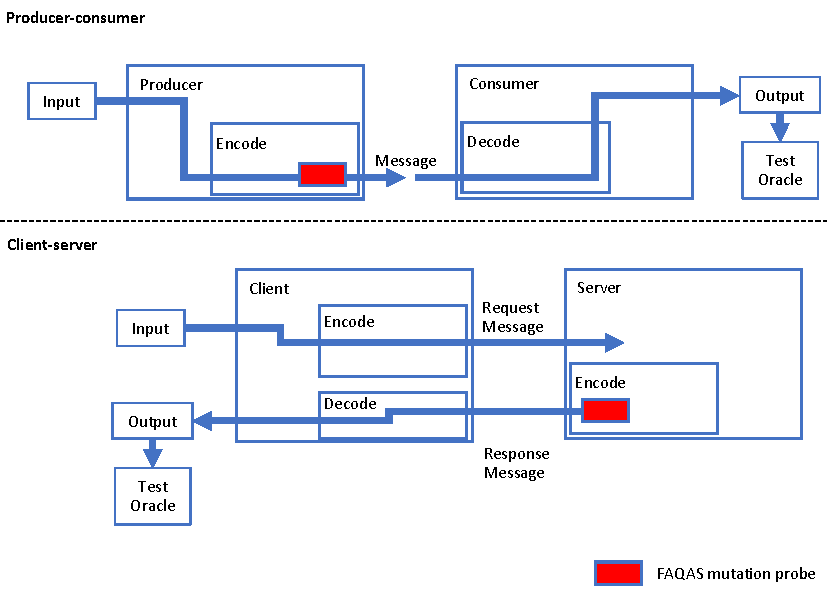
\includegraphics[width=14cm]{images/dataDrivenTestSuiteAugmentationC}
      \caption{Data-driven mutation analysis for different architectures.}
      \label{fig:dataDrivenTestSuiteAugmentationC}
\end{figure}

\begin{figure}[h]
  \centering
    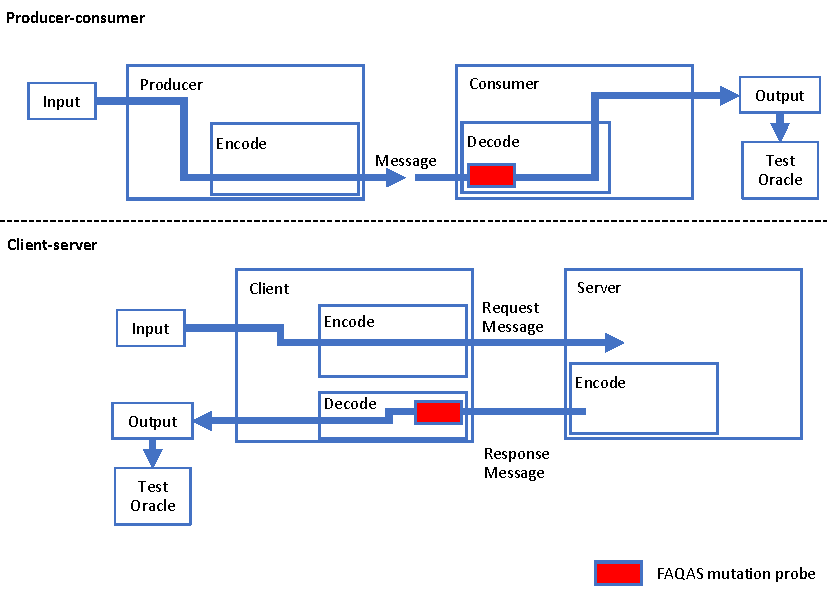
\includegraphics[width=14cm]{images/dataDrivenTestSuiteAugmentationD}
      \caption{Data-driven mutation analysis for different architectures.}
      \label{fig:dataDrivenTestSuiteAugmentationD}
\end{figure}

\begin{figure}[h]
  \centering
    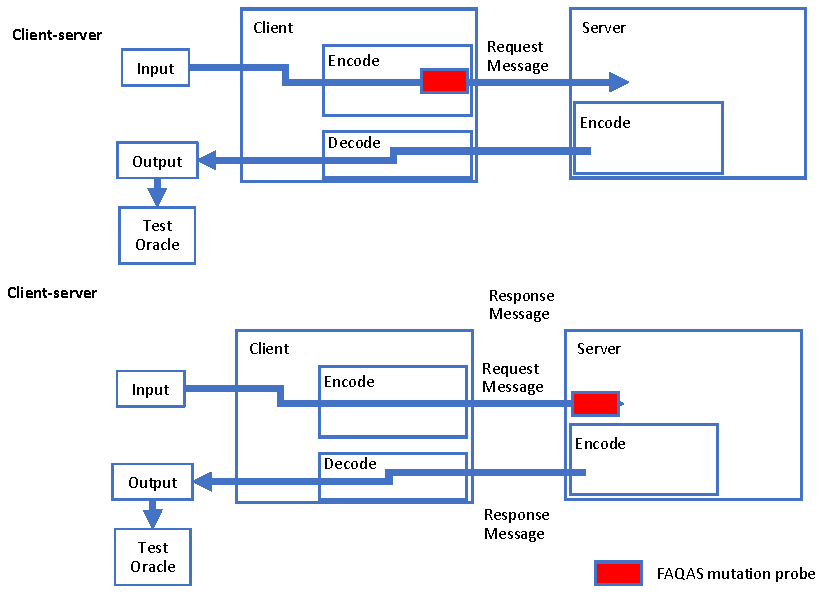
\includegraphics[width=14cm]{images/dataDrivenTestSuiteAugmentationE}
      \caption{Data-driven mutation analysis for different architectures.}
      \label{fig:dataDrivenTestSuiteAugmentationE}
\end{figure}

\begin{figure}[h]
  \centering
    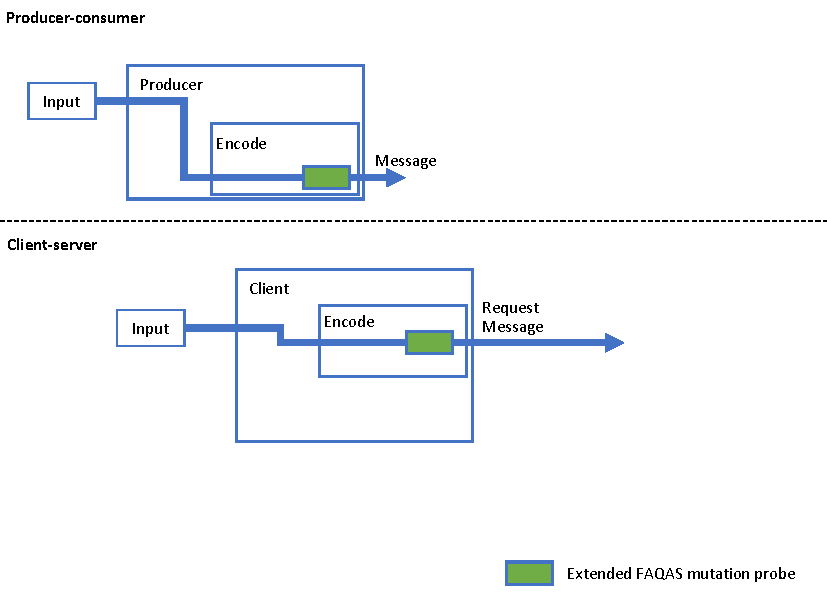
\includegraphics[width=14cm]{images/dataDrivenTestSuiteAugmentationB}
      \caption{Data-driven mutation analysis for different architectures.}
      \label{fig:dataDrivenTestSuiteAugmentationB}
\end{figure}

\ENDCHANGEDWPT



\clearpage
\subsection{Test generation with a client-server system}

\STARTCHANGEDWPT

For our example, we rely on the libParam case study provided by GSL. Listing~\ref{GSLmutate} shows the mutation probe, which is inserted into function \emph{gs\_rparam\_process\_packet}, on the server side. The probe mutates the buffer \emph{v\_General}, which contains a copy of a message request (i.e., \emph{request}). In the case of GSL, the FVAT operator configured to mutate \emph{request-$\>$table\_id} cannot be applied (i.e., MOC is not equal to 100\%); this indicates that the test cases do not cover a scenario in which the client passes a \emph{table\_id} above the threshold. To generate such a test case we may rely on the extended probe combined with \INDEX{static program analysis}. 

Listing~\ref{GSLcover} shows how the \INDEX{extended mutation probe} might be inserted into the code of libParam. In practice, it requires the engineer to know the portion of code that handles the generation of a request message. Unfortunately, injecting the mutation probe is not sufficient to enable test generation but engineers need also to prepare a test template to enable test generation with KLEE. Listing~\ref{GSLtest} shows an example of such template based on existing libParam test cases; such test case requires the initialization of a number of state variables, which limits the possibility to automate its definition. For this reason, within FAQAS we did not find it feasible to automate data-driven mutation analysis with a tool but we aim to evaluate its manual feasibility in WP4.

Finally, when data-driven mutation is applied to the data generated by the server, test automation is made unfeasible by the fact that KLEE cannot work in the presence of a communication channel within the code to be analyzed. Such shortcoming is not observed when we mutate request data because the extended mutation probe is installed only on the client; the producer-consumer case is not affected by such shortcoming because, in this case, the probe is installed on the producer. Alternative test generation tools or extensions of KLEE shall be considered to overcome such limitations.

% !TEX root =  ../MAIN.tex
\begin{lstlisting}[style=CStyle, caption=Example of data-driven mutation probe for libParam, label=GSLmutate]

static void gs_rparam_process_packet(csp_conn_t * conn, csp_packet_t * request_packet)
{
    csp_packet_t * reply_packet = NULL;
    gs_rparam_query_t * reply;


    /* Handle endian */
    gs_rparam_query_t * request = (gs_rparam_query_t *) request_packet->data;


    request->length = csp_ntoh16(request->length);
    request->checksum = csp_ntoh16(request->checksum);


    FaultModel *fm_General = _FAQAS_General_FM();
    unsigned long long int v_General[6];

    v_General[0] = (unsigned long long int) request->action;
    v_General[1] = (unsigned long long int) request->table_id;
    v_General[2] = (unsigned long long int) request->length;
    v_General[3] = (unsigned long long int) request->checksum;
    v_General[4] = (unsigned long long int) request->seq;
    v_General[5] = (unsigned long long int) request->total;


    _FAQAS_mutate(v_General,fm_General);
    
\end{lstlisting}



%flag E_Decode(E* pVal, BitStream* pBitStrm, int* pErrCode)
%{
%    flag ret = TRUE;
%    *pErrCode = 0;
%    (void)pVal;
%    (void)pBitStrm;
%
%
%    (*(pVal))=5; ret = TRUE; *pErrCode = 0;
%
%    // Manually added probe 
%    E_mutate(pVal);
%    // Manually added probe END
%    return ret  && E_IsConstraintValid(pVal, pErrCode);
%}


% !TEX root =  ../MAIN.tex
\begin{lstlisting}[style=CStyle, caption=Example of extended data-driven mutation probe for libParam, label=GSLcover]

/**
   Get string.
   @note If the returned string is max length, the value buffer will not be 0 terminated.
   @param[in] node CSP address
   @param[in] table_id remote table id.
   @param[in] addr parameter address (remote table).
   @param[in] checksum checksum
   @param[in] timeout_ms timeout
   @param[out] value returned value (user allocated)
   @param[in] value_size size of \a value, i.e. size of parameter type in bytes.
   @return_gs_error_t
*/
static inline gs_error_t gs_rparam_get_string(uint8_t node, gs_param_table_id_t table_id, uint16_t addr,
                                              uint16_t checksum, uint32_t timeout_ms, char * value, size_t value_size)
{
    return gs_rparam_get(node, table_id, addr, GS_PARAM_STRING, checksum, timeout_ms, value, value_size);
}


gs_error_t gs_rparam_get(uint8_t node,
                         gs_param_table_id_t table_id,
                         uint16_t addr,
                         gs_param_type_t type,
                         uint16_t checksum,
                         uint32_t timeout_ms,
                         void * value,
                         size_t value_element_size)
{
    return gs_rparam_get_array(node, table_id, addr, type, checksum, timeout_ms, value, value_element_size, 1);
}


gs_error_t gs_rparam_get_array(uint8_t node,
                               gs_param_table_id_t table_id,
                               uint16_t addr,
                               gs_param_type_t type,
                               uint16_t checksum,
                               uint32_t timeout_ms,
                               void * value,
                               size_t value_element_size,
                               size_t array_size)
{
    /* Calculate length */
    gs_rparam_query_t * query;
    const size_t query_payload_size = sizeof(query->payload.addr[0]) * array_size;
    const size_t query_size = RPARAM_QUERY_LENGTH(query, query_payload_size);
    const size_t reply_payload_element_size = value_element_size + sizeof(query->payload.addr[0]);
    const size_t reply_payload_size = reply_payload_element_size * array_size;
    const size_t reply_size = RPARAM_QUERY_LENGTH(query, reply_payload_size);

    query = alloca(reply_size);
    query->action = RPARAM_GET;
    query->table_id = table_id;
    query->checksum = csp_hton16(checksum);
    query->seq = 0;
    query->total = 0;
    for(unsigned int i = 0; i < array_size; i++) {
        query->payload.addr[i] = csp_hton16(addr + (value_element_size * i));
    }
    query->length = csp_hton16(query_payload_size);

    FaultModel *fm_General = _FAQAS_General_FM();
    unsigned long long int v_General[6];

    v_General[0] = (unsigned long long int) query->action;
    v_General[1] = (unsigned long long int) query->table_id;
    v_General[2] = (unsigned long long int) query->length;
    v_General[3] = (unsigned long long int) query->checksum;
    v_General[4] = (unsigned long long int) query->seq;
    v_General[5] = (unsigned long long int) query->total;


    _FAQAS_cover(v_General,fm_General);


    /* Run single packet transaction */
    if (csp_transaction2(CSP_PRIO_HIGH, node, GS_CSP_PORT_RPARAM, timeout_ms, query, query_size, query, reply_size, CSP_O_CRC32) <= 0) {
        return GS_ERROR_IO;
    }
 ... 
 
 }

\end{lstlisting}



%flag E_Decode(E* pVal, BitStream* pBitStrm, int* pErrCode)
%{
%    flag ret = TRUE;
%    *pErrCode = 0;
%    (void)pVal;
%    (void)pBitStrm;
%
%
%    (*(pVal))=5; ret = TRUE; *pErrCode = 0;
%
%    // Manually added probe 
%    E_mutate(pVal);
%    // Manually added probe END
%    return ret  && E_IsConstraintValid(pVal, pErrCode);
%}


% !TEX root =  ../MAIN.tex
\begin{lstlisting}[style=CStyle, caption=Test template to enable data-driven mutation testing for libParam, label=GSLtest]

    // a little hack - this is next element, we use it check for overwrite and missing 0 termiation
    memset(alltypes_mem.string_A, 'Z', sizeof(alltypes_mem.string_A));
    alltypes_mem.string_A[0][1] = 0;

    char buf[GS_TEST_ALLTYPES_STRING_LENGTH + 10];

    // get max size - no 0 termination
    memset(alltypes_mem.string, 'B', sizeof(alltypes_mem.string));
    memset(buf, 'A', sizeof(buf));
    buf[GS_TEST_ALLTYPES_STRING_LENGTH + 1] = 0;
    
    csp_node CSP_NODE;
    unsigned long long int tableID;
    klee_make_symbolic(&CSP_NODE, sizeof(CSP_NODE), "CSP_NODE");
    klee_make_symbolic(&tableID, sizeof(tableID), "tableID");
    gs_rparam_get_string(&CSP_NODE, tableID, GS_TEST_ALLTYPES_STRING, GS_RPARAM_MAGIC_CHECKSUM, 1000, buf, GS_TEST_ALLTYPES_STRING_LENGTH);

    
\end{lstlisting}



%flag E_Decode(E* pVal, BitStream* pBitStrm, int* pErrCode)
%{
%    flag ret = TRUE;
%    *pErrCode = 0;
%    (void)pVal;
%    (void)pBitStrm;
%
%
%    (*(pVal))=5; ret = TRUE; *pErrCode = 0;
%
%    // Manually added probe 
%    E_mutate(pVal);
%    // Manually added probe END
%    return ret  && E_IsConstraintValid(pVal, pErrCode);
%}


\ENDCHANGEDWPT



